On a recent work trip to London, I had the privilege of attending a
LondonFurs meet, which I have to say was spectacular. There's not really
an analog around where I am, though I imagine the meet known only to me
as ``Chicken'' in California might come close. It was big - hovering
around 50 or so people - and there were a good percentage of the
attendees in suit, which was new to me. In Northern Colorado, we don't
have too much in the way of furmeets, and what we do are quiet, intimate
affairs with maybe 15 attendees, tops. Suiting happens, but is uncommon,
and tends to represent only a small portion of the furries in
attendance.

\begin{figure}[htbp]
\centering
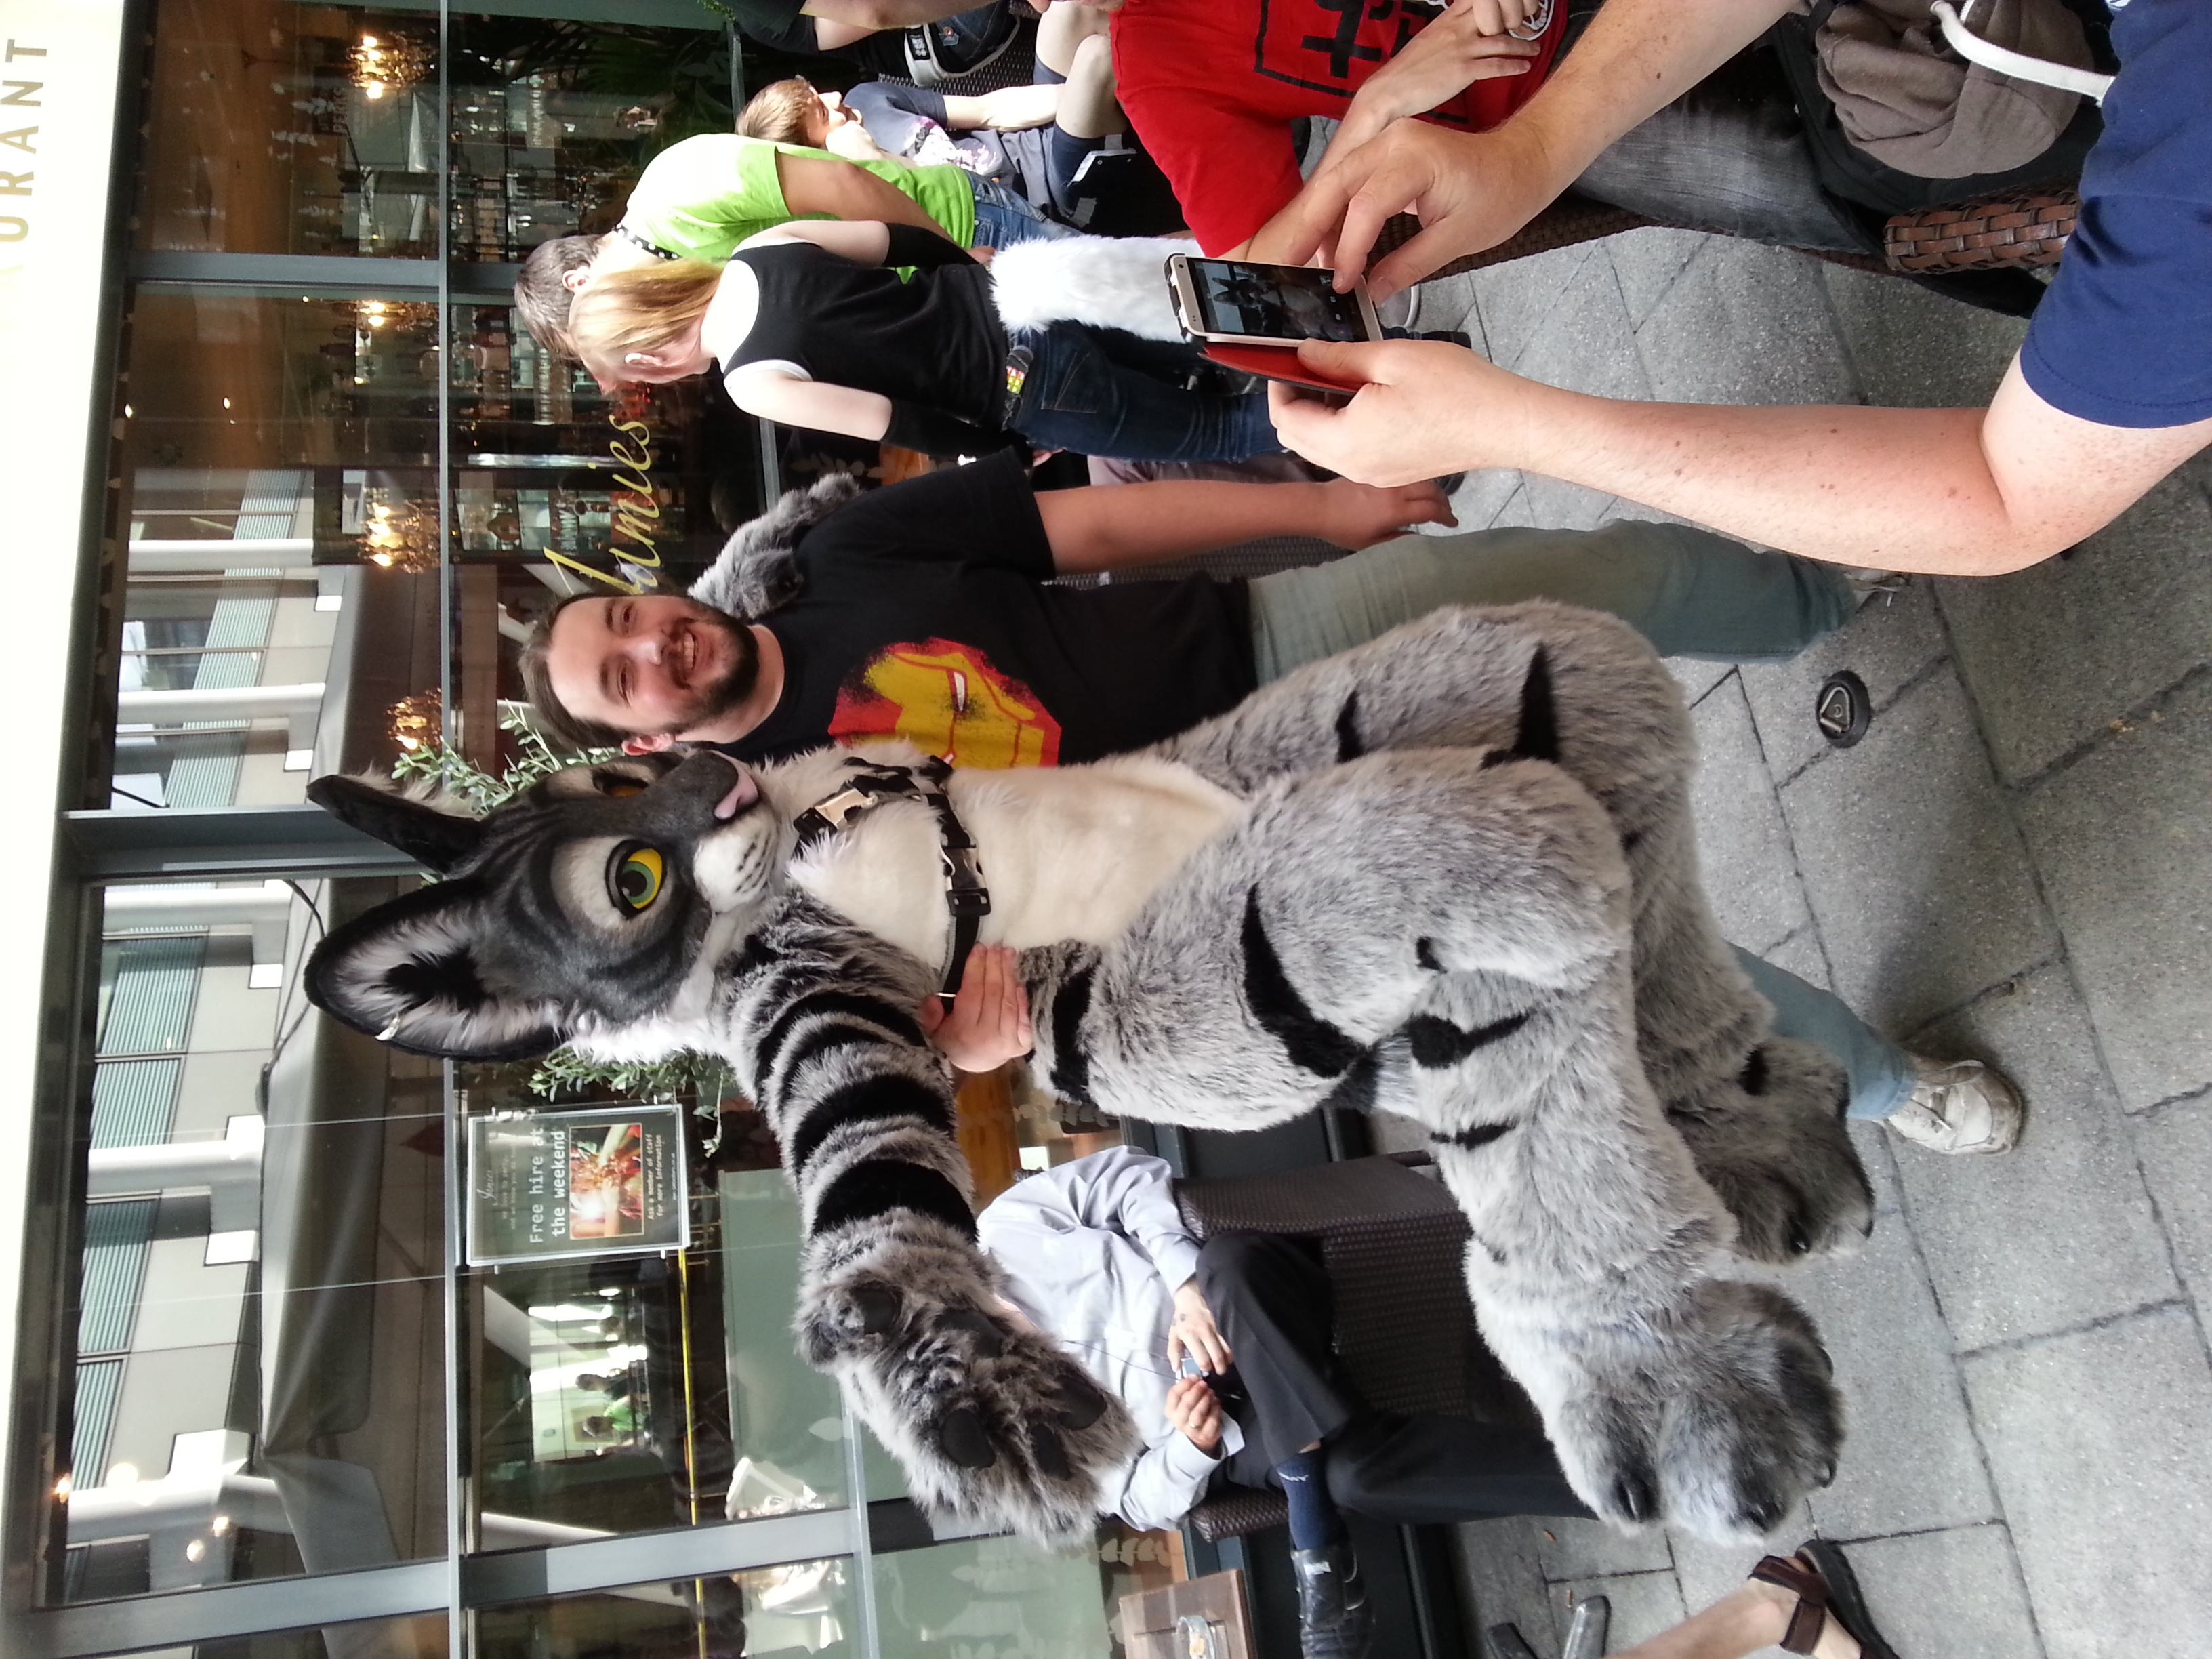
\includegraphics{/assets/furry/play-in-furry/01.jpg}
\caption{}
\end{figure}

Another interesting thing was the barrier-to-entry in that the meet took
place at a city bar, and thus attracted an older crowd, at least of
drinking age (though note JM's
\href{http://adjectivespecies.com/2014/08/18/reflections-on-an-american-furry-convention/}{recent
comment} that this includes furries 18 years old and older, rather than
21 as it would be in the United States).

As I sipped mediocre cocktails (seriously, how hard is it to make a
Pimm's?!) and aggressively pink wines, I noticed a common trend among
the furries - notably among the fursuiters: playfulness. Childish,
simple playfulness. This, I think, is something of a universal within
our fandom: the tendency toward play.

Play, commonly seen as an activity that takes place between children, or
between children and a facilitating adult such as a parent, is an
important part of development, particularly in the development of a
child's psychology. Play itself serves many purposes during a child's
intellectual development and helps to provide a strong basis for the
growth of the individual. Outdoor play, for instance, helps to
strengthen a child's connection to and understanding of the environment
around them. Meanwhile, social play can help solidify language within
the growing child and lay the foundation for learning as the individual
progresses through school (thus why play is seen as an integral part of
early education).

Play also helps to solidify social interaction between individuals.
Pretend play and other types of social play are formative in the ways in
which children interact with each other into adulthood. Additionally,
there is a strong emotional component to play. Childhood psychologists
and therapists have often used play as a way of interacting with
children on an emotional level. In short, play helps to shape the whole
of the child's personality.

\begin{figure}[htbp]
\centering

\includegraphics{/assets/furry/play-in-furry/02.jpg}
\caption{}
\end{figure}

The play that I witnessed at that LondonFurs meet, the one that struck
me with the idea for this article, was simple. Three furries - two in
suit, one out of suit - had arrayed themselves in an equilateral
triangle and were rolling a swirly-green beach ball back and forth.
Occasionally, the ball would escape the trio, and, with much visible
consternation, one of the fursuiters would go scrambling after it and
gleefully bring it back to the small circle. Onlookers watched and
laughed, some took pictures, and everyone seemed to be enjoying
themselves.

This type of scene seemed to me to be particularly furry. That is to
say, it was notable in how common it was. It's not uncommon to see
furries engaging in playful activities, especially in suit - it was one
of the \href{https://www.youtube.com/watch?v=PMFdVIE3Zj0}{first things}
I did when I got mine. It's a common sight, seeing furries and
fursuiters playing around at conventions, almost to the point where it
seems out of place seeing a fursuiter not hamming it up and simply
striding purposefully toward some goal.

On the surface, this raises quite a few questions. What exactly is the
reason for this focus on play within furry. Is it a type of
infantilization? That is, are we intentionally acting more childlike in
order to feel more childlike ourselves? Or perhaps it's a type of
reclaimed innocence. We act like children in order to relive more
childlike (and thus perceived as more fun) portions of our lives. Or
perhaps it's simply a means of letting down one's ``front-stage
persona'' in the Erving Goffman sense: we're showing who we truly are -
playful individuals - without the professional and interpersonal masks
that we otherwise keep firmly in place.

\begin{figure}[htbp]
\centering
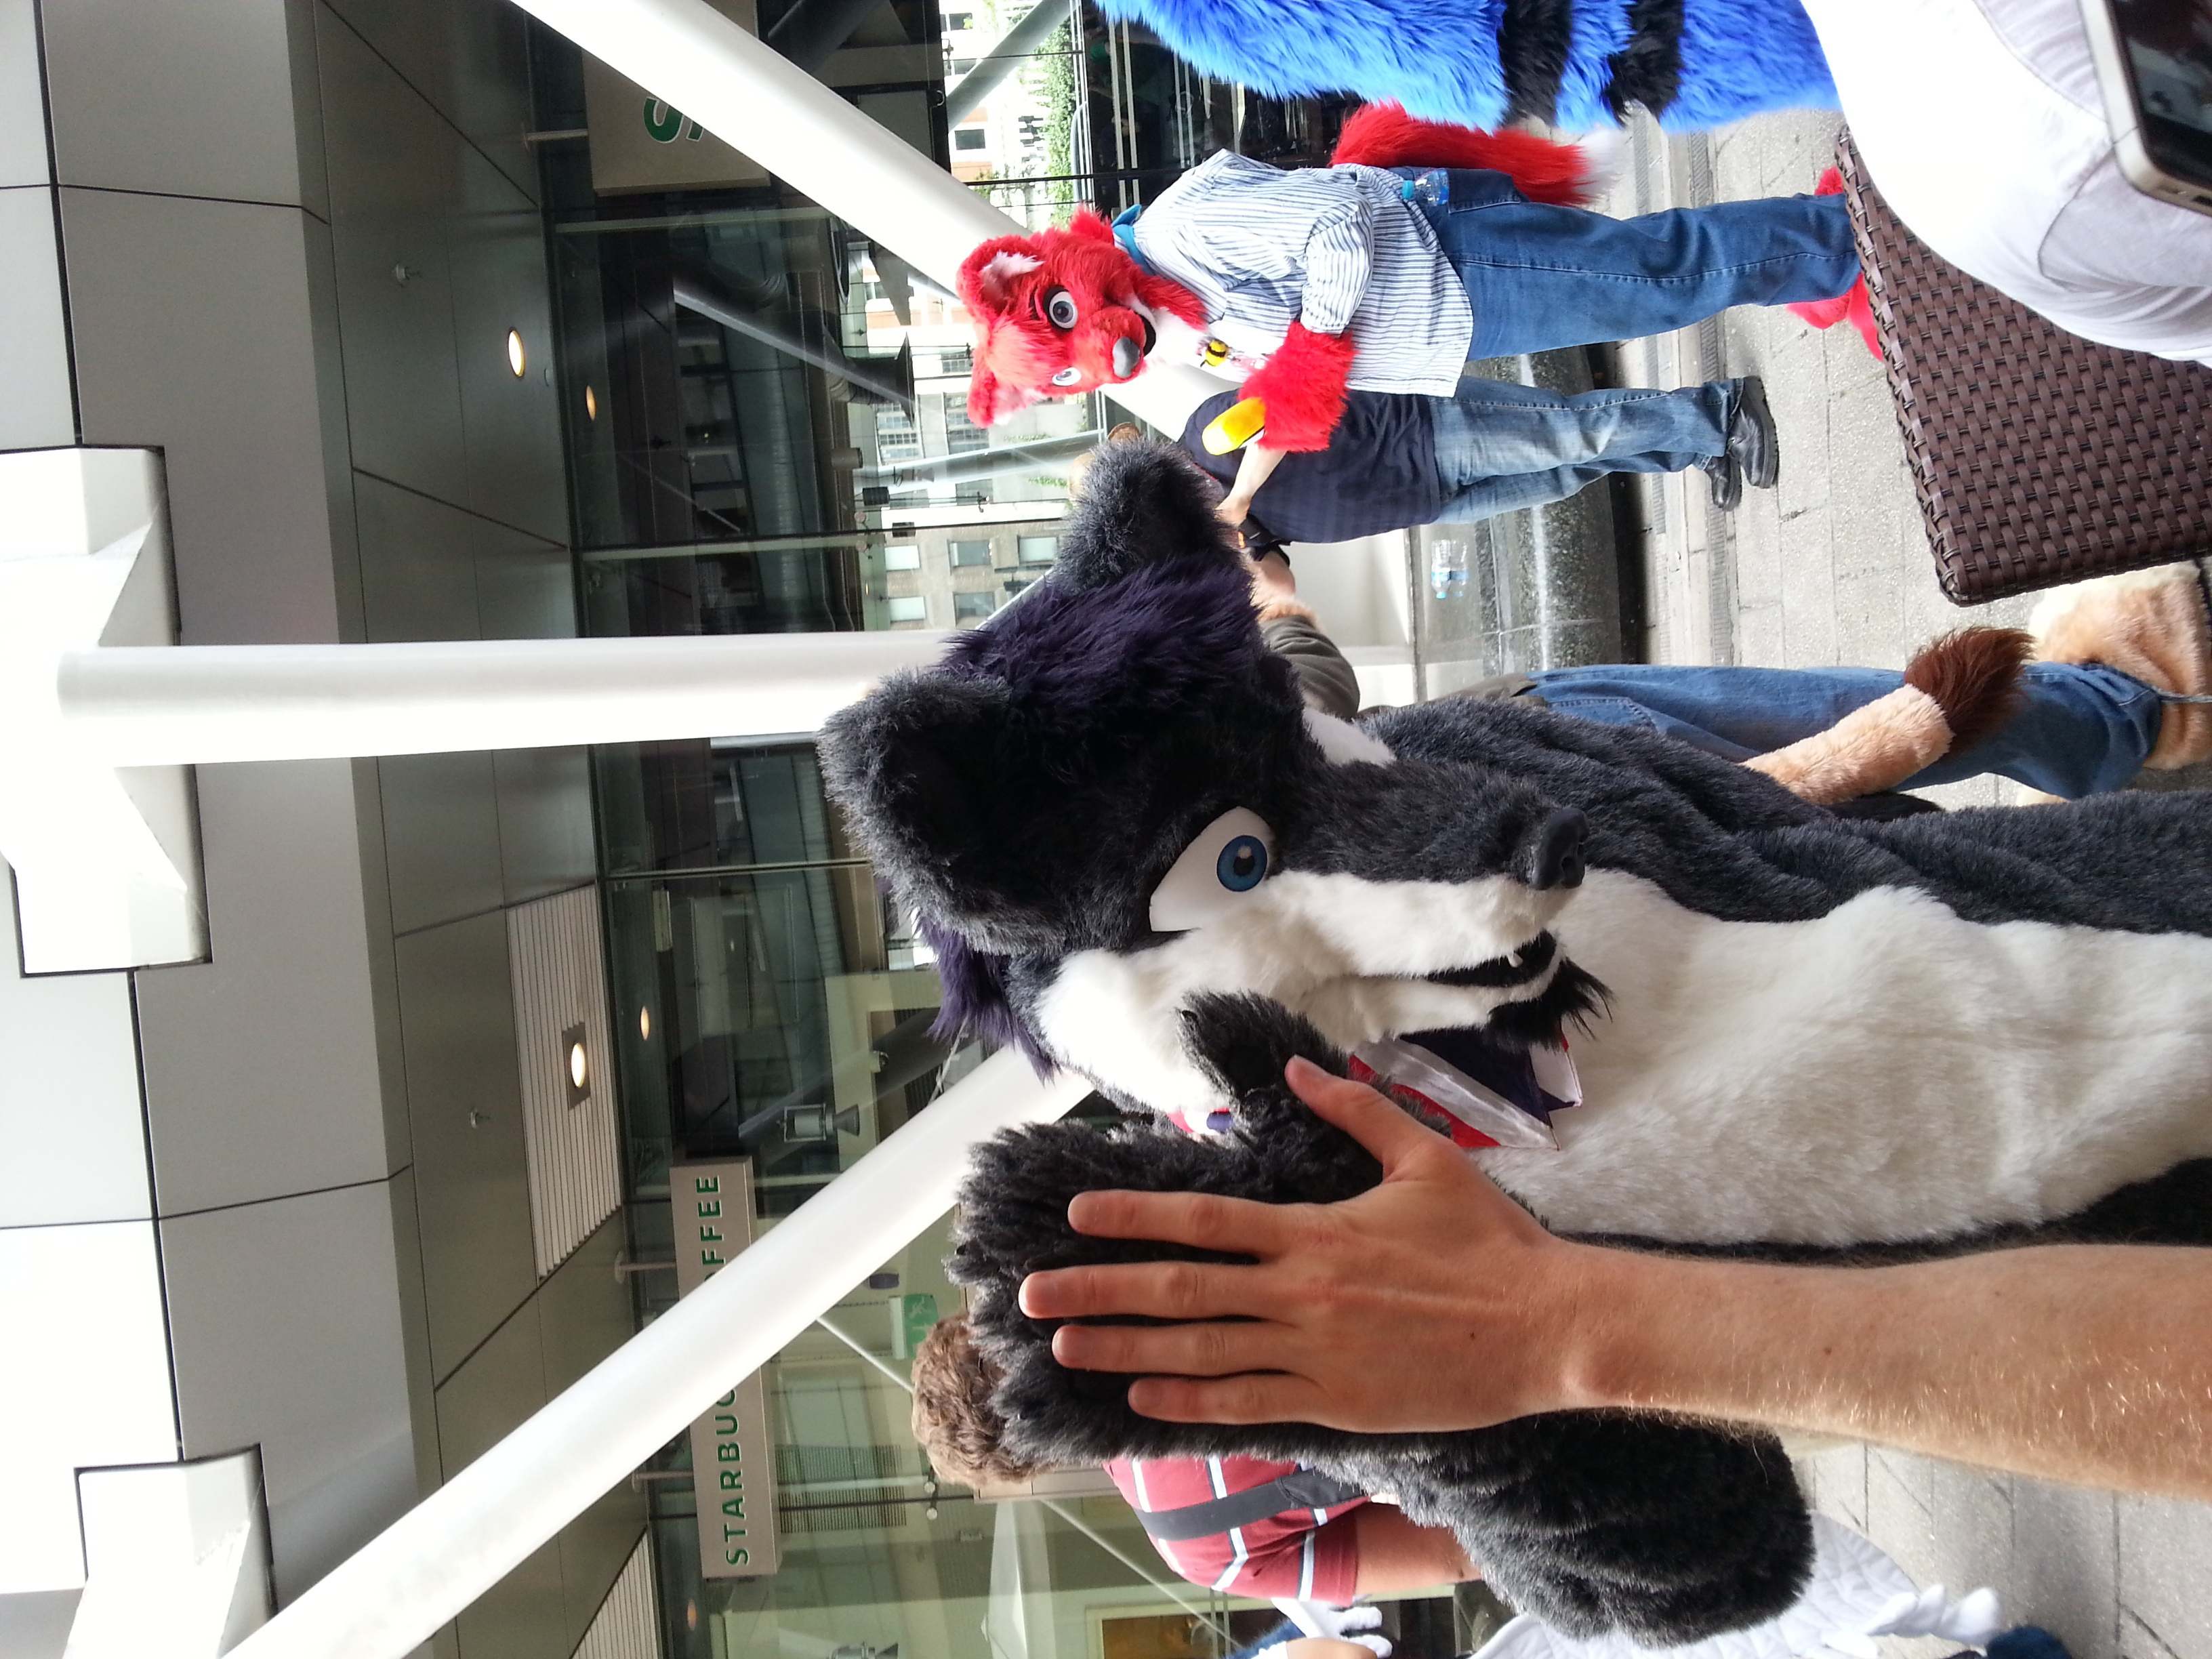
\includegraphics{/assets/furry/play-in-furry/03.jpg}
\caption{}
\end{figure}

With that last bit in mind, it's worth noting that, in adults, play
plays a slightly different role than in children. It's associated most
often with a strength of character found primarily in humor, teamwork,
and creativity. There are various aspects of playfulness that all adults
exhibit throughout their lives, and for various reasons, as mentioned.
Playfulness is a healthy thing for adults to experience, as well as
children, and there are aspects of it that fit in all of our day-to-day
lives. {[}\href{http://www.psywb.com/content/1/1/4}{ref}{]}

I think this is all quite important to furry, and not just due to the
prevalence. I think that playfulness and childishness inform furry on a
more fundamental level than we honestly give them credit for. I know the
common refrain that furry is about hearkening back to our
Saturday-morning-cartoon childhoods, that fursuiting is something we do
for the enjoyment of children, and I believe that truly is the case for
some, but I think that frames the whole situation in a much less
personal, much more selfless way. At heart, I think the truth is that a
good many of us truly are playful. Our childishness isn't something
that's immature, as this playfulness even shows up in our more adult
creations, but it's something that shows our strength of character.
After all, not only are we able to maintain a mask with which we
interact with the public and professional world, but we are also able to
let that down and interact with each other through true, honest play.
